%%%%%%%%%%%%%%%%%%%%%%%%%%%%%%%%%%%%%%%%%%%%%%%%%%%%%%


\section{Soft-Collinear Effective Theory}\label{sec:SCET}
%https://arxiv.org/pdf/1410.1892.pdf


Below the factorization structure of the double differential jet production cross section is displayed in the context of Soft-Collinear Effective Theory, SCET, following the framework for inclusive jet production $pp \rightarrow jet + X$ developed in for jets of  %https://arxiv.org/abs/1801.00790

\begin{equation}
\frac{d \sigma}{ d p_{T} d m}=\sum_{a b c} f_{a}\left(x_{a}, \mu\right) \otimes f_{b}\left(x_{b}, \mu\right) \otimes H_{a b}^{c}\left(x_{a}, x_{b}, p_{T} / z, \mu\right) \otimes \mathcal{G}_{c}\left(z, p_{T} R, m, \mu, z_{\mathrm{cut}}, \beta\right)
\end{equation}
% equation from here https://arxiv.org/pdf/1811.06983.pdf

Jet and Soft Functions 


Image of factorization in this context

%SCET-factorization
~\cite{Becher:2014oda}
%https://arxiv.org/abs/1410.1892
\begin{figure}[htb]
\centering
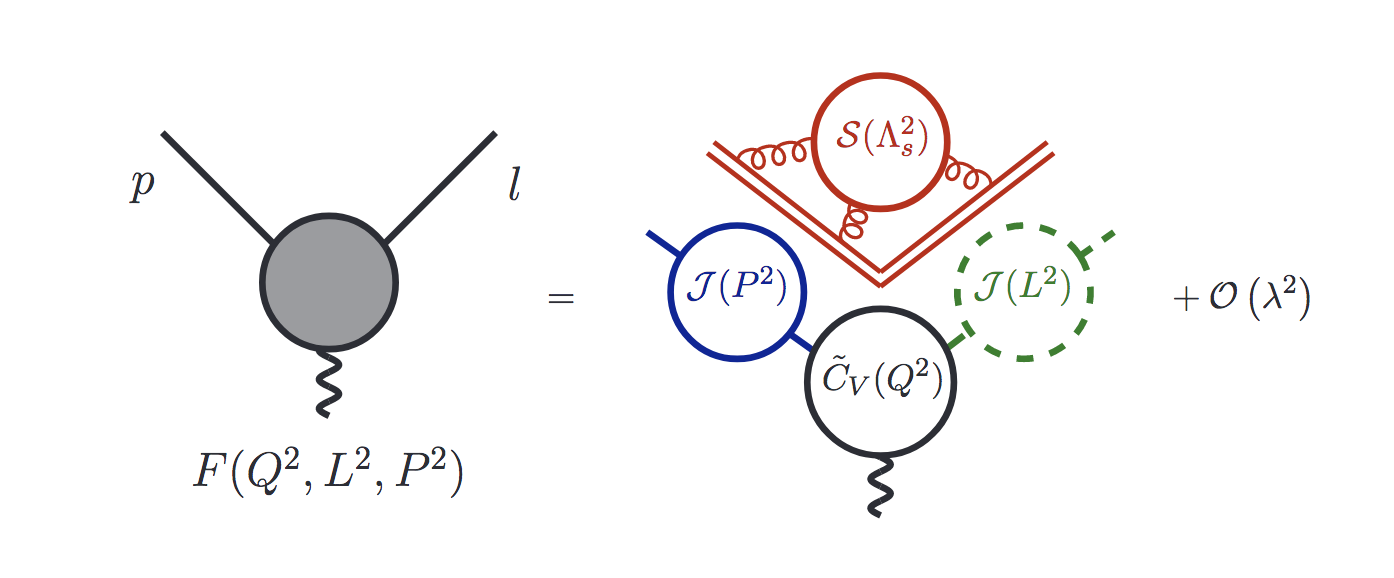
\includegraphics[width=1.0\textwidth]{visuals/SCET-factorization.png}
\caption{Fatorization of the energy scales in a hard scatter interaction according to SCET ~\cite{Becher:2014oda}.}
\label{fig:scet}
\end{figure}
discuss groomed jets in this context

comparing groomed  (Jet) to ungroomed (Jet+Soft)


%%%%%%%%%%%%%%%%%%%%%%%%%%%%%%%%%%%%%%%%%%%%%%%%%%%%%%%%%%%%%%%%%%%%%%%%%%%%%%%%%%%%%%%%%%%%%%

\section{Jets Initited by Quarks and Gluons }\label{sec:quarkandgluonjets}



%earlier discussed $C_F = \frac{4}{3}$ and $C_A=3$ 

%CITE A Theory of Quark vs. Gluon Discrimination
% https://arxiv.org/pdf/1906.01639.pdf

%Dijets make quark gluon admixture %cite SMP-16-10
%Z+Jets make mostly light quark jets, studied here and in 7 TeV analysis (1 D unfolding there and no soft drop)

% http://cms-results.web.cern.ch/cms-results/public-results/publications/SMP-16-010/index.html




% ATLAS thesis http://inspirehep.net/record/1672323/files/2016_Mantifel_PhD_Atlas_Z.pdf

In order to emphasize the relevance to the measurement presented herein, the phenomenology of Quantum Chromodynamics is discussed rather than the Lagrangian perspective. This is useful as jet studies help probe QCD in the soft and collinear limits. 
% https://arxiv.org/pdf/1709.06195.pdf CITE THIS LECTURE
Jets are formed by the hadronization of quarks and gluons. In this thesis I present a measurement of a light quark enriched jet sample. 



Consider the simplest process that could produce a quark initiated jet, a quark of energy $E_q$  emitting a gluon of energy $E_g$. The probability that this will occur is a function of the gluon's energy fraction, $z$, and the emission angle , $\theta$  \cite{Larkoski:2017fip}.\newline


$z = \frac{E_g}{E_q + E_g}$\newline

$1 - cos \theta = \frac{m^2}{2 E_q E_g}$\newline

Then the probability of gluon emission from the quark is :


$P_q(z,cos \theta) dz d cos \theta = \frac{\alpha_s C_F}{\pi}  \frac{dz}{z} \frac{dcos \theta}{1 - cos \theta}  $\newline

It is useful to assume the small angle approximation, $\theta << 1$, giving:\newline


$P_q(z,\theta^2) dz d \theta^2 = \frac{\alpha_s C_F}{\pi}  \frac{dz}{z} \frac{d \theta^2}{ \theta^2}  $\newline

Notice that the probability of emission diverges for very soft (small z) or very collinear (small $\theta$) gluons. In the soft and collinear limits the probability can be interpretted as an expectation value for the number of soft/collinear gluons \cite{Larkoski:2017fip}.

It is elucidating to rewite the probability in terms of inverse logarithms in the and introduce the "Lund Diagram" in order to visualize the uniform distribution of soft and collinear gluons in the $log \frac{1}{ \theta^2} , log\frac{1}{z} $ space.

\begin{figure}[htb]
\label{fig:lund}
\centering
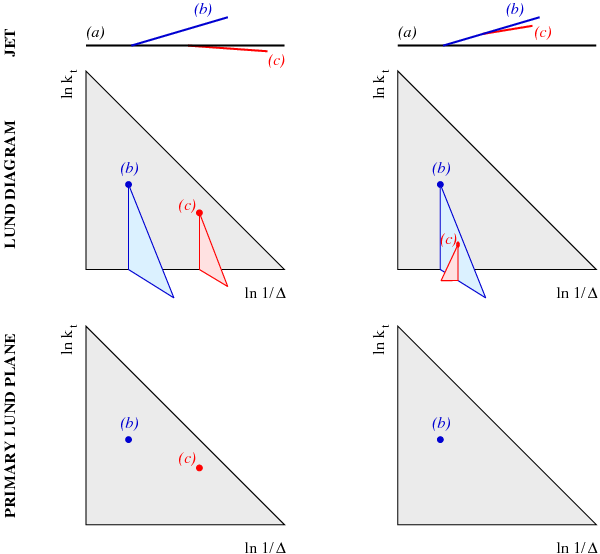
\includegraphics[width=1.0\textwidth]{visuals/figs_lund.png}
\caption{The primary and secondary lund planes for 2 example jets~\cite{Dreyer:2018nbf}.}

\end{figure}


The primary lund plane is shown in Figure ~/ref{fig:lund} ~\cite{Dreyer:2018nbf}
%image 



$P_q(z,\theta^2) dz d \theta^2 = \frac{\alpha_s C_F}{\pi} d( log\frac{1}{z}  ) d(log \frac{1}{ \theta^2})  $\newline

At leading order (LO) jets can also be "initiated" by gluons and this probability is incredibly similar :


$P_q(z,\theta^2) dz d \theta^2 = \frac{\alpha_s C_A}{\pi} d( log\frac{1}{z}  ) d(log \frac{1}{ \theta^2})  $\newline


This similarity allows us to interpret the variations in quark enriched and gluon enriched jet samples in terms of the fundamental $C_F$ and adjoint $C_A$ casimirs, in $SU(3)$ ,   $C_F = \frac{4}{3}$ and $C_A=3$. This is also the only difference between quark and gluon jet masses at LO as shown in ~\ref{sec:jetmass}.


Comparing the probability of a quark to emit a gluon and that of a gluon to to emit a gluon, we can see the ratio is simply $\frac{C_A}{C_F} =\frac{9}{4} $. This has strong experimental implications since it implies gluon jets will on average be composed of about twice as many constituent particles as quark jets, and will be broader. This will cause gluon jets to have higher mass, since the mass of a $1 \rightarrow 2 $ splitting is given by $\theta \simeq \frac{2}{\gamma} $, this is derived in ~\ref{chap:RelativisticKinematics},.




